\documentclass[11pt, a4paper]{article}

\usepackage[margin=2.1cm]{geometry}
\usepackage[utf8]{inputenc}
\usepackage[T1]{fontenc}
\usepackage[spanish]{babel}
\usepackage{array}
\usepackage{booktabs}
\usepackage{caption}
\usepackage{float}
\usepackage{graphicx}
\usepackage{hyperref}
\usepackage{xcolor}

\definecolor{cjcblue}{RGB}{31,97,169}

\setlength{\parindent}{0pt}
\setlength{\parskip}{6pt}
\setlength{\textfloatsep}{10pt plus 2pt minus 2pt}
\setlength{\floatsep}{8pt plus 2pt minus 2pt}
\renewcommand{\arraystretch}{1.08}
\captionsetup{font=normalsize, labelfont=bf}
\graphicspath{{Paper/figures/}{figures/}}
\hypersetup{colorlinks=true, urlcolor=cjcblue, linkcolor=black}
\addto\captionsspanish{\renewcommand{\tablename}{Cuadro}}

\begin{document}

\begin{center}

\includegraphics[width=0.30\textwidth]{logo_cjc_palatino_horizontal.png}

\textbf{Comunicado de prensa}

Centro Javeriano de Competitividad \textbar{} Pontificia Universidad Javeriana
\end{center}

{\color{cjcblue}\rule{\textwidth}{0.8pt}}

\begin{center}
%{\Large\bfseries Colombia creció más por tener más ocupados que por aumentar su productividad entre 2010 y 2025}
{\Large\bfseries El crecimiento económico de Colombia ha dependido más del aumento del empleo que del aumento de la productividad}
\vspace{4pt}

\begin{minipage}{0.96\textwidth}
\begin{list}{\textbullet}{%
  \setlength{\leftmargin}{1.2em}
  \setlength{\labelwidth}{0.8em}
  \setlength{\labelsep}{0.4em}
  \setlength{\itemsep}{3pt}
  \setlength{\topsep}{2pt}
}
  \item \textbf{La productividad laboral cayó en actividades como los servicios públicos, la minería y la construcción.}
  \item \textbf{En el agregado nacional, el PIB por hora trabajada creció 1,5\% anual, pero las horas semanales promedio por trabajador cayeron 0,5\% anual.}
  \item \textbf{Por esa razón, el PIB por trabajador aumentó apenas 1,1\% anual, frente a un crecimiento del PIB real de 3,2\%.}
  \item \textbf{El contraste muestra que el crecimiento económico dependió más de tener más personas ocupadas que de producir más por trabajador.}
\end{list}
\end{minipage}

\vspace{8pt}

Bogotá, 30 de junio de 2026.

\end{center}

%Un nuevo informe del \textbf{Centro Javeriano de Competitividad} muestra que el crecimiento del país provino más de la expansión del número de ocupados que de un aumento del producto por trabajador. El informe, titulado \textbf{Dinámicas de la Productividad Laboral por Actividad Económica en Colombia 2010--2025}, calcula la evolución del \textbf{producto por trabajador} y del \textbf{producto por hora trabajada}, tanto para el agregado nacional como para las principales ramas de actividad económica.

\textbf{Entre 2010 y 2025, Colombia aumentó su PIB principalmente porque más personas estuvieron ocupadas, no porque la producción por trabajador creciera al mismo ritmo.} Según un nuevo informe del Centro Javeriano de Competitividad, los ocupados crecieron 2,1\% anual, mientras que el PIB por trabajador aumentó 1,1\% anual. El resultado muestra que el país ha sostenido buena parte de su crecimiento en la expansión del empleo, pero todavía enfrenta un reto persistente de productividad.

%\textbf{Entre 2010 y 2025, el número de personas ocupadas aumentó 2,1\% anual, mientras que el PIB por trabajador creció 1,1\% anual.} Por lo tanto, cerca de dos de los poco más de tres puntos porcentuales de crecimiento anual del PIB se explican por el aumento de la población ocupada y el resto por el aumento del producto por trabajador.

%\textbf{En el mismo periodo, el PIB por hora trabajada creció 1,5\% anual, pero las horas semanales promedio por trabajador disminuyeron 0,5\% anual.} Esa caída en las horas trabajadas explica por qué el PIB por trabajador creció menos que el PIB por hora trabajada. Por lo tanto, parte de la ganancia en productividad por hora se tradujo en más tiempo disponible fuera del trabajo, una mejora de bienestar que no queda capturada por el aumento de los ingresos.

\textbf{En el mismo periodo, el PIB por hora trabajada creció 1,5\% anual, pero las horas semanales promedio por trabajador disminuyeron 0,5\% anual.} Esa caída en las horas trabajadas explica por qué el PIB por trabajador creció menos que el PIB por hora trabajada. Por lo tanto, parte de la ganancia en productividad por hora se tradujo en menos horas trabajadas, lo que en algunos casos puede reflejar una mejora de bienestar que no queda capturada por el aumento de los ingresos.

\textbf{La caída de las horas trabajadas enmascara la contribución del aumento de la productividad por hora al crecimiento del PIB.} El crecimiento anual del PIB real (3,2\%) se explica, de forma aproximada, por el aumento de los ocupados (2,1\%), la caída en las horas trabajadas por ocupado (-0,5\%) y el crecimiento del PIB por hora trabajada (1,5\%). Esta descomposición se resume en la Figura \ref{fig:comunicado_descomposicion}.

\textbf{El informe alerta sobre caídas de productividad en varias actividades económicas entre 2010 y 2025.} En crecimiento del PIB por trabajador, las actividades con mayores aumentos fueron: 1. arte, entretenimiento, recreación y otros servicios (7,3\% anual); 2. información y comunicaciones (3,7\%); y 3. agropecuario (2,8\%). En contraste, las mayores caídas se registraron en: 1. servicios públicos (-3,8\% anual); 2. minas (-3,6\%); y 3. construcción (-3,1\%). 

\textbf{El informe advierte, sin embargo, que las actividades donde la productividad creció más no necesariamente son las actividades con mayores niveles de productividad.} Por ejemplo, el sector agropecuario registró uno de los mayores avances, pero sigue siendo uno de los de menor productividad laboral en la economía. El Cuadro \ref{tab:comunicado_productividad_sector} presenta la evolución de la productividad por hora y por trabajador de cada actividad.

%\textbf{El informe advierte, sin embargo, que las actividades donde la productividad creció más no necesariamente son las actividades con mayores niveles de productividad.} Por ejemplo, aunque el sector agropecuario aumentó significativamente su productividad, todavía se encuentra rezagado en su nivel de productividad relativo al resto de la economía. El Cuadro \ref{tab:comunicado_productividad_sector} presenta la evolución de la productividad por hora y por trabajador de cada actividad.

\textbf{\textit{``La agenda del país debe identificar los obstáculos que han frenado el crecimiento de la productividad de ciertos sectores, así como los factores que han dinamizado a otros''}}, señala Oliver Pardo, Director del Centro Javeriano de Competitividad.

\textbf{Descargue y consulte el informe \href{https://github.com/oliverpardo1979/Informe_Actividades/raw/main/Outputs/Informe_01_20260619.pdf}{aquí}.}. Contáctenos en \href{mailto:cjce@javeriana.edu.co}{cjce@javeriana.edu.co}.


\begin{figure}[H]
  \centering
  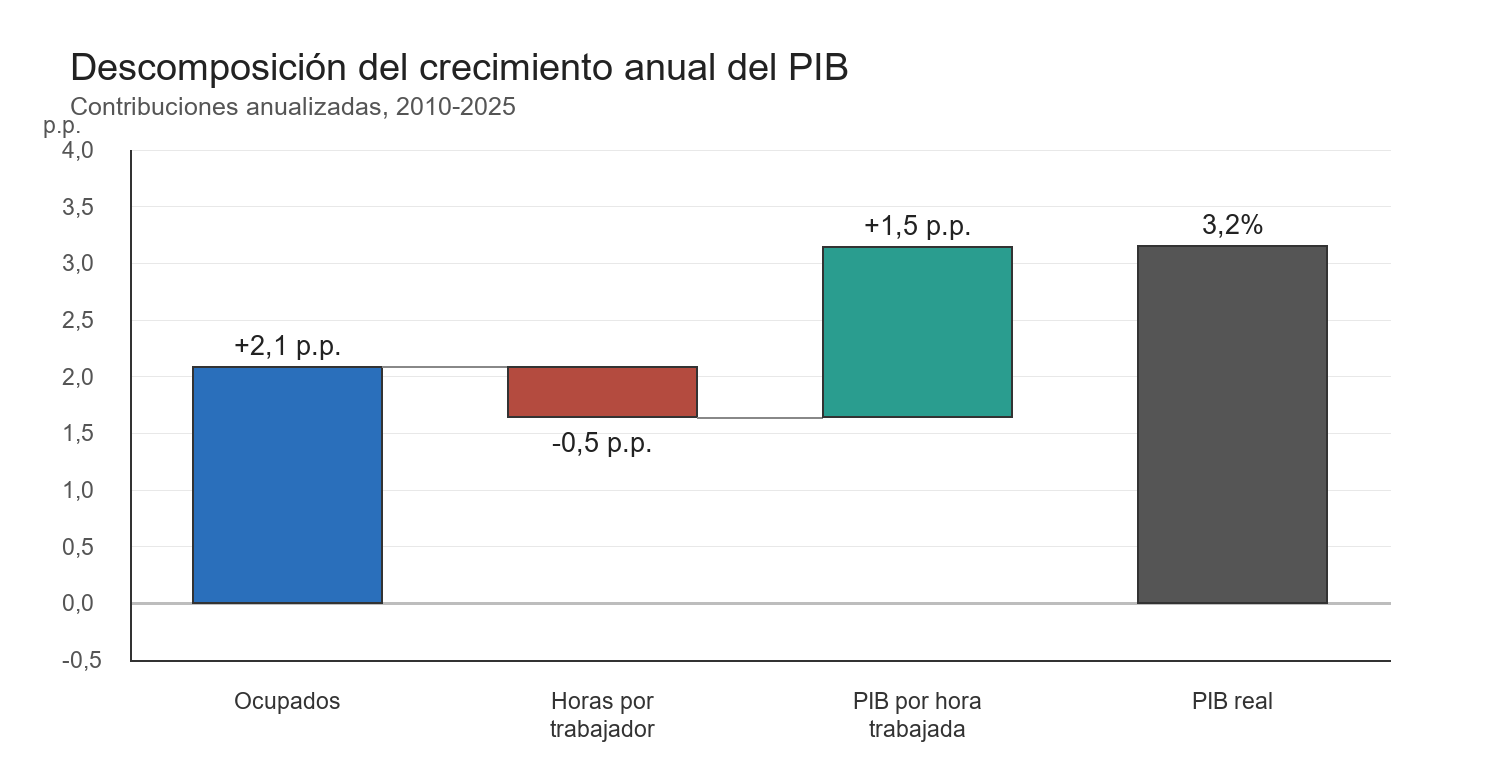
\includegraphics[width=0.82\textwidth]{fig_pib_geih_descomposicion_crecimiento_comunicado.png}
  \caption{Descomposición del crecimiento anual del PIB, 2010--2025}
  \label{fig:comunicado_descomposicion}
  \caption*{Nota: las barras intermedias muestran cuánto aporta cada componente, en puntos porcentuales, al crecimiento anualizado del PIB real. Fuente: cálculos propios con base en Cuentas Nacionales y GEIH del DANE.}
\end{figure}

\begin{table}[H]
\centering
\caption{Productividad laboral por actividad económica, 2010--2025}
\label{tab:comunicado_productividad_sector}
\setlength{\tabcolsep}{4pt}
\begin{tabular}{>{\raggedright\arraybackslash}p{5.4cm}rrrrrr}
\toprule
& \multicolumn{3}{c}{PIB por trabajador} & \multicolumn{3}{c}{PIB por hora} \\
& \multicolumn{3}{c}{Millones de pesos de 2015} & \multicolumn{3}{c}{Miles de pesos de 2015} \\
\cmidrule(lr){2-4}\cmidrule(lr){5-7}
Actividad económica & 2010 & 2025 & Crec. & 2010 & 2025 & Crec. \\
\midrule
Arte, recreación y otros servicios & 11,4 & 32,8 & 7,3\% & 5,6 & 16,0 & 7,3\% \\
Información y comunicaciones & 45,4 & 78,6 & 3,7\% & 17,6 & 34,0 & 4,5\% \\
Agropecuario & 13,5 & 20,4 & 2,8\% & 5,8 & 9,4 & 3,3\% \\
Hogares como empleadores & 6,4 & 9,4 & 2,6\% & 2,7 & 4,5 & 3,5\% \\
Adm. pública, educación y salud & 43,9 & 58,4 & 1,9\% & 19,5 & 26,1 & 2,0\% \\
Financieras & 101,0 & 124,5 & 1,4\% & 43,0 & 54,2 & 1,6\% \\
Comercio, transporte y alojamiento & 20,9 & 24,1 & 1,0\% & 7,9 & 10,1 & 1,6\% \\
Manufactura & 40,1 & 45,0 & 0,8\% & 16,5 & 19,5 & 1,1\% \\
Inmobiliarias & 280,0 & 284,6 & 0,1\% & 105,3 & 119,5 & 0,9\% \\
Profesionales y administrativas & 54,3 & 42,4 & -1,6\% & 24,8 & 20,6 & -1,2\% \\
Construcción & 41,8 & 26,1 & -3,1\% & 16,4 & 11,0 & -2,6\% \\
Minas & 200,8 & 115,8 & -3,6\% & 77,6 & 48,4 & -3,1\% \\
Servicios públicos & 176,5 & 99,5 & -3,8\% & 70,0 & 43,5 & -3,1\% \\
\bottomrule
\end{tabular}
\caption*{Nota: las actividades están ordenadas por el crecimiento anual del PIB por trabajador. Fuente: cálculos propios con DANE y GEIH.}
\end{table}

%{\color{cjcblue}\rule{\textwidth}{0.6pt}}

\end{document}
